\documentclass[../draft.tex]{subfiles}

\begin{document}
    \chapter{Theory}\label{c:theory}
    In the first part of this chapter, we define the flow functions for the IFDS analysis. In the second part, we discuss taint analysis's runtime, highlighting possible differences between forward and backward analysis.

    \section{Flow Functions}\label{s:flowfunctions}
    We describe the flow functions' behavior based on the Jimple language and define semi-formal rules analogous to the publication\cite{Arzt2017PhD} on \textsc{FlowDroid}. These rules only focus on the basic language constructs. We describe flows for additional language features such as arrays and exceptions later and more informal in \autoref{s:rules}.

    \subsection{Normal Flow}\label{s:normalflow}
    Normal flow functions handle every statement that does not contain an \code{InvokeExpr}.
    % and assignments are always explicit in Jimple.
    For the base cases in normal flow, new taints are only produced at assignments. Assignments are always explicit in Jimple and are either \code{AssignStmt}s or \code{IdentityStmt}s. The \code{IdentityStmt}'s are at the top of a method\footnote{With the exception of \footnotecode{local_name := @caughtexception}, which is outside of the base cases.} and assign special values to locals, e.g., parameters and the \code{this} reference. We perform the identity function over those because we want to keep those taints alive to reach the return edge. Then the Return Flow function takes care of mapping all parameters back into the caller\footnote{Note that traversing the interprocedural control-flow graph backward means call edges are now return edges and vice versa.}. So in the following, we only consider \code{AssignStmt}s.

    Now, let us consider an \code{AssignStmt} where the left side is either a field reference or a local and the right side is an expression.
    In the following, we assume the right side is always a local or a field dereference.
    If the expression is an \code{InvokeExpr}, we handle this in the call flow.
    For unary operators, the local can simply be extracted and for binary operators, we consider both locals separately.
    An assignment has the structure $x.f^n \leftarrow y.g^m$ with $n,m \in \{0,1\}$ modeling a possible field reference.
    As taints may have an access path of an arbitrary length, we denote this as $h^k$.\footnote{$h^k$ is a $k$-length chain of field dereferences, not $k$-times the same field dereference}
    Jimple also ensures only one field dereference per statement, which Arzt chose not to represent in the semi-formal definitions and neither did we.

    In the first case, we look at exact matches. Either we have an assignment with a local ($n=0$) or a field dereference ($n=1$). For both, the base variable needs to match. For the latter, also the first field of the access path has to match the field dereference.
    The first field dereference is removed from the taint and the remaining access path is copied to the newly created taint. The incoming taint is killed because, thinking forward, it received the taint at this statement.
    \begin{itemize}
        \item[] \textbf{Rule 1:} An incoming taint $T = x.f^n.h^k$ with $k \geq 0$ produces the outflowing taint set $\left\{y.g^m.h^k\right\}$.
    \end{itemize}
    % Rule 1 work likewise with a wildcard appended after $h^k$. Similiary to the rest access path $h^k$, it is copied to the right side.

    Next, we need a rule for the case the field dereference $f$ is included in a cut-off approximation.
    Recall \autoref{s:ap}, symbolic access paths can also be $k$-limited to speedup the analysis and are $k=5$-limited in \textsc{FlowDroid} by default.
    Thus, we might encounter a taint with no field dereferences and a wildcard $*$ appended.
    In this case, just the base needs to match.
    However, this time, the left side is kept alive because we can not reason which field is tainted due to the cut-off approximation.
    \begin{itemize}
        \item[] \textbf{Rule 2:} An incoming taint $T = x.*$ with $k \geq 0$ produces the outflowing taint set $\left\{y.g^m.*, T\right\}$.
    \end{itemize}

    Whenever a taint does not match the left side, we perform the identity as the statement does not touch the tainted variable's contents.
    Later on, when we consider aliasing, there is one special case inside the default case.
    If the tainted variable is on the right side, an additional alias query is needed.
    We reference this case in \autoref{s:aliasing}.

    \subsection{Call Flow}
    The Call Flow function and subsequently Return and Call To Return Flow function apply whenever a statement contains an \code{InvokeExpr}.
    For call statements without an assignment, we have statements of the structure $o.m(a_0, ..., a_n)$ with $n \in \mathbb{N}$. $a_i$ denotes the $i$-th argument, $p_i$ the corresponding parameter to $a_i$ and $c$ the class instance of the callee's base object.

    When we encounter a tainted argument in the caller, the taint needs to go through the callee.
    Java uses pass-by-value\footnotemark{}.
    \footnotetext{
        According to the Java specification, arguments are always \textit{values} (Source: \url{https://docs.oracle.com/javase/specs/jls/se11/html/jls-8.html\#jls-8.4.1} (visited on 19.05.2021)).
        Thus, many argue that Java is strictly pass-by-value.
        Sometimes reference types are described as pass-by-reference because the behavior of those is similar to what pass-by-reference is.
        The ambiguity is owed to the time when the term pass-by-reference was defined. 
        Back then, 23 year before Java was invented, reference was used to describe an address in the memory \cite{Fairley1973}.
        A precise description of the semantics is given in the following lines.
    }
    Thus, for primitives, the value is copied and pushed on the stack.
    For reference types, the reference to the object is copied and pushed on the stack.
    Resulting, the callee can change the field values on the reference and those changes are reflected in the caller but it can not alter the reference the caller operates on.
    Now, if only the reference is tainted but nothing more ($k=0$ and no wildcard), an update to the tainted reference in the callee has no effect on the tainted argument in the caller.
    We know because of these semantics in combination with the backward direction that a tainted primitive or reference without field dereferences can not originate from inside the callee.
    This property becomes apparent when we get specific to Java's types.
    Primitives do not have fields and strings are immutable\footnote{The special handling of strings results in transparent fields, e.g. we can treat strings as if they were primitives in this case.}.
    Consider the example in \autoref{lst:primret}.
    On the left, we use the built-in String type.
    In line 2, \code{str} is copied into \code{callee}.
    After this statement, both \code{str} hold the value \code{42} but point to another memory location\footnotemark{}.
    \footnotetext{%
        The JVM might only set a copy-on-write flag on \footnotecode{str} in \footnotecode{callee} and point it to the identical location as \footnotecode{str} in \footnotecode{main} to save memory.
        At least right before the update happens, it is guaranteed that the variable points to a different location.
    }
    Thus, \code{main} carries on with the original value of \code{str} no matter what \code{callee} writes to \code{str}.
    In contrast, on the right, the callee can update the field on the heap.
    Therefore, the taint needs to be propagated into the callee to find the leak.
    Conclusively, $k$ needs to be greater than $0$.
    \begin{itemize}
        \item[] \textbf{Rule 1:} An incoming taint $T=a_i.h^k$ with $k > 0 \land 0 \leq i \leq n$ produces the outflowing taint set $\left\{p_i.h^k\right\}$.
        \item[] \textbf{Rule 2:} An incoming taint $T=a_i.*$ with $0 \leq i \leq n$ produces the outflowing taint set $\left\{p_i.*\right\}$.
    \end{itemize}

    \begin{figure}[tbp]
        \centering
        \begin{subfigure}[b]{0.45\textwidth}
            \centering
            \begin{adjustbox}{max width=\columnwidth}
                \begin{lstlisting}[gobble=20]
                    void main() {
                        String str = "42";
                        callee(str);
                        sink(str); // no leak
                    }

                    void callee(String str) {
                        str = source();
                    }
                \end{lstlisting}
            \end{adjustbox}
            \caption{Taint Without Fields}
        \end{subfigure}
        \qquad
        \begin{subfigure}[b]{0.45\textwidth}
            \centering
            \begin{adjustbox}{max width=\columnwidth}
                \begin{lstlisting}[gobble=20]
                    void main() {
                        SomeObject o = new SomeObject();
                        callee(o);
                        sink(o.str); // leak
                    }

                    void callee(SomeObject o) {
                        o.str = source();
                    }
                \end{lstlisting}
            \end{adjustbox}
            \caption{Taint With Fields}
        \end{subfigure}
        \caption{Call Flow Example}
        \label{lst:primret}
    \end{figure}

    A non-static callee can also access instance fields of the base object.
    When we observe a tainted base object, the taint also needs to flow through the callee.
    The tainted object transforms into a $\mathit{this}$ reference.
    In Java, \code{this} references the current instance the method operates on.
    \begin{itemize}
        \item[] \textbf{Rule 3:} An incoming taint $T=o.h^k$ with $k > 0$ produces the outflowing taint set $\left\{\mathit{this}_c.h^k\right\}$.
        \item[] \textbf{Rule 4:} An incoming taint $T=o.*$ produces the outflowing taint set $\left\{\mathit{this}_c.*\right\}$.
    \end{itemize}

    Static fields form a special case.
    Their scope extends over the whole program and thus, tainted static fields always have to go through the callee.
    The taint is untouched as the access to those is the same everywhere.
    \begin{itemize}
        \item[] \textbf{Rule 5:} An incoming taint $T = S.f.h^k$ with $k \geq 0$ produces the outflowing taint set $\left\{T\right\}$.
    \end{itemize}

    In Jimple, \code{AssignStmt}s can also consist of an \code{InvokeExpr} on the right side.
    The structure of the statement is in this case $x \leftarrow o.m(a_0,...,a_n)$. $r_i$ denotes a return value.
    $n_r$ is the number of return statements in the callee.
    If we observe such a statement and the left side is tainted, we need to map the left-hand side of the \code{AssignStmt} back into the callee.
    Now, methods can have multiple return statements and as we traverse the reversed interprocedural control-flow graph, there are multiple outgoing edges.
    We can not reason which return statement is the right one, so we need to taint every return statement's operand in the callee.
    \begin{itemize}
        \item[] \textbf{Rule 6:} An incoming taint $T = x.h^k$ with $k \geq 0$ produces the outflowing taint set $\left\{r_i.h^k \mid 0 \leq i < n_r \right\}$.
    \end{itemize}

    Unlike at normal flows, we kill all taints not matching any of the rules.
    In the case of a taint being out of the callee's scope, the Call To Return flow function propagates the taint over the statement.

    \subsection{Return Flow}
    Taints reaching the end of a method need to be mapped back into the caller.
    The statement we consider is of the structure $o.m(a_0, ..., a_n)$ with $n \in \mathbb{N}$.
    Again, $a_i$ denotes the $i$-th argument, $p_i$ the $i$-th parameter and $c$ the class instance.

    The first rule is the counterpart rule 1 and 2 of Call Flow\footnotemark{} and map all parameters back into the caller.
    \footnotetext{Note that if $k$ can be $0$, the wildcard also works.}
    In contrast to the Call Flow, we also map primitives and strings back into the caller.
    When a taint reaches the end of a method in the backward interprocedural control-flow graph, it is actually at the start of the method.
    At the start of a method, the contents of a tainted parameter were copied from the caller.
    Thus we taint the argument in the caller.
    \begin{itemize}
        \item[] \textbf{Rule 1:} An incoming taint $T = p_i.h^k$ with $k \geq 0 \land 0 \leq i \leq n$ produces the outflowing taint set $\{a_i.h^k\}$.
    \end{itemize}

    The $\mathit{this}$ reference also needs to be mapped back into the caller.
    \begin{itemize}
        \item[] \textbf{Rule 2:} An incoming taint $T = \mathit{this}_c.h^k$ with $k \geq 0$ produces the outflowing taint set $\{o.h^k\}$.
        \item[] \textbf{Rule 3:} An incoming taint $T = \mathit{this}_c.*$ with $k \geq 0$ produces the outflowing taint set $\{o.*\}$.
    \end{itemize}

    Tainted static fields are also mapped back. As already written in the corresponding rule 5 of Call flow, the taint is untouched.
    \begin{itemize}
        \item[] \textbf{Rule 4:} An incoming taint $T = S.h^k$ with $k \geq 0$ produces the outflowing taint set $\{T\}$.
    \end{itemize}

    Again, taints not matching any rule are killed.
    For example, this kills taints, which are not in the caller's scope, when returning from a method.

    \subsection{CallToReturn Flow}
    The statement structure is $o.m(a_0, ..., a_n)$ with $n \in \mathbb{N}$.
    $a_i$ denotes the $i$-th argument.

    A taint is independent of a callee if it is not static and neither matches an argument nor the base object the method is called on.
    Such a taint is not matched inside Call Flow and needs to be propagated over the call statement.
    \begin{itemize}
        \item[] \textbf{Rule 1:} An incoming taint $x.h^k$ with $k \geq 0 \land \left(\forall i \in [0, n] \cap \mathbb{N}: a_i \neq x\right) \land x \neq o \land x \notin \mathit{StaticVariables}$ produces the outflowing taint set $\{T\}$.
    \end{itemize}

    Now, consider again the left side of \autoref{lst:primret}.
    In line 3, the \code{str} taint is in the kill set of Call Flow because the callee can not be responsible for the tainted variable in the caller.
    Nevertheless, the taint is still valid after the call.
    As we want to preserve the taint, we need to propagate the taint over the call statement in such cases.
    \begin{itemize}
        \item[] \textbf{Rule 2:} An incoming taint $T = a_i$ with $0 \leq i \leq n$ produces the outflowing taint set $\{T\}$.
    \end{itemize}

    Like in Call and Return Flow, we also kill taints that do not match any of these rules.

    \section{Runtime of the Data Flow Analysis}\label{s:complexity}
    IFDS has a worst-case time complexity of $O(|E| \cdot |D|^3)$ \cite{Reps1995}. $|E|$ is the number of observed edges in the control-flow graph and $|D|$ is the number of observed domain elements by the IFDS analysis.
    Consequently, the complexity highly depends on the analyzed app and the location of the sources or sinks, depending on the analysis direction.
    Therefore it is not possible to deduce a general advantage for any direction.
    Nevertheless, there are certain cases where one direction is favorable, which we discuss in the following paragraphs.

    We decide favorably based on the number of taint propagations, i.e., the exploded supergraphs observed edges.
    They correlate to the runtime and depend on two factors: taints' lifetime and the number of taints.
    In the following paragraphs, we show examples where the analysis direction influences both factors.
    After that, we discuss clues suitable for an apriori decision on the direction.

    \begin{figure}[tbp]
        \centering
        \begin{adjustbox}{max width=\textwidth}
            \begin{lstlisting}[gobble=16]
                String returnParam(int i, String s1, String s2, String s3) {
                    if (i == 1)
                        return s1;
                    else if (i == 2)
                        return s2;
                    else if (i == 3)
                        return s3;
                    else
                        return "default";
                }
            \end{lstlisting}
        \end{adjustbox}
        \caption{Call Flow Rule 6 Example}
        \label{lst:branching}
    \end{figure}

    First, we take a look at the branching factor.
    The branching factor describes the number of outgoing edges from a node.
    A smaller branching factor is favorable.
    Consider a binary operator expression such as \code{int c = a + b;}.
    Backward, we can not argue which operand is responsible for the tainted output and thus proceed with both operands tainted.
    The same restriction is present in rule 6 of Call Flow which describes how the returned value is mapped back into the callee.
    This time the branching factor can be even larger.
    For example, in \autoref{lst:branching} is a method that conditionally returns one of its parameters and is part of the leak path.
    Let us assume the returned value of a call to \code{returnParam()} is tainted. Backward, every returned operand is tainted and later on mapped according to Return Flow rule 2 back into the caller.
    The effect gets apparent when looking at the method summary.
    The IFDS algorithm ends up with a summary $\mathit{retVal} \rightarrow \{s1, s2, s3\}$.
    Forward, a tainted parameter is mapped into the callee and later on returned to the caller resulting in three possible summaries  $s1 \rightarrow \mathit\{\mathit{retVal}, s1\}$, $s2 \rightarrow \mathit\{\mathit{retVal}, s2\}$ or $s3 \rightarrow \mathit\{\mathit{retVal}, s3\}$.
    Such a case favors the forward analysis.

    In contrast, a strict right-to-left flow favors backward analysis as taints are killed more often due to a stricter overwrite rule.
    In \autoref{tikz:rtol} is such a right-to-left flow displayed.
    Forward, the right-hand side is always kept alive because it still holds the tainted value below the statement and could be leaked.
    When traversing a right-to-left flow backward, the left side is always killed.
    A visited statement is the update responsible for tainting, leading to a branching factor of 1 and a shorter lifetime per taint.\\
    A prominent real-world example of a right-to-left order is Java's \code{StringBuilder}.
    The implementations of \code{append()} and \code{insert()} return the \code{this} instance to allow for easy chaining of multiple calls.
    Consider the corresponding Jimple code in \autoref{lst:stringbuilder}.
    Soot does not reuse the local variables when translating JVM bytecode to Jimple\footnotemark{}.
    \footnotetext{Locals are reused when converting Dalvik bytecode to Jimple.}
    Although all locals from \code{\$stack9} to \code{\$stack15} refer to the same object, the forward analysis can not kill any of those.
    In a simple view, our backward analysis has a huge advantage here.
    However, when we also consider aliases, the advantage is weakened by the aliasing queries.
    Nevertheless, because the Java compiler internally transforms non-constant string concatenation into a \code{StringBuilder}, \code{StringBuilder} objects are present in nearly every JVM-based program.

    \begin{figure}[tbp]
        \centering
        \begin{subfigure}[b]{0.45\textwidth}
            \centering
            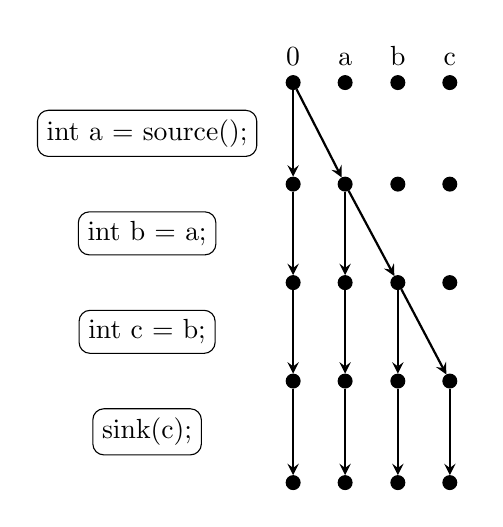
\begin{tikzpicture}[auto,
                s/.style={draw, rounded corners},
                v/.style={draw, fill=black, circle, inner sep=0pt, minimum size=5pt},
                every node/.style={align=center},
                every matrix/.style={ampersand replacement=\&,column sep=0.25cm,row sep=.25cm},
                vto/.style={->, >=stealth, thick}]
                \matrix {
                    \& \node[v, label=0] (zero1) {}; \& \node[v, label=a] (a1) {}; \& \node[v, label=b] (b1) {}; \& \node[v, label=c] (c1) {};\\
                    \node[s] (s1) {\smallcode{int a = source();}}; \& \& \& \&\\
                    \& \node[v] (zero2) {}; \& \node[v] (a2) {}; \& \node[v] (b2) {}; \& \node[v] (c2) {};\\
                    \node[s] (s2) {\smallcode{int b = a;}}; \& \& \& \&\\
                    \& \node[v] (zero3) {}; \& \node[v] (a3) {}; \& \node[v] (b3) {}; \& \node[v] (c3) {};\\
                    \node[s] (s3) {\smallcode{int c = b;}}; \& \& \& \&\\
                    \& \node[v] (zero4) {}; \& \node[v] (a4) {}; \& \node[v] (b4) {}; \& \node[v] (c4) {};\\
                    \node[s] (s4) {\smallcode{sink(c);}}; \& \& \& \&\\
                    \& \node[v] (zero5) {}; \& \node[v] (a5) {}; \& \node[v] (b5) {}; \& \node[v] (c5) {};\\
                };

                \draw[vto] (zero1) -- (zero2);
                \draw[vto] (zero2) -- (zero3);
                \draw[vto] (zero3) -- (zero4);
                \draw[vto] (zero4) -- (zero5);

                \draw[vto] (zero1) -- (a2);
                \draw[vto] (a2) -- (a3);
                \draw[vto] (a3) -- (a4);
                \draw[vto] (a4) -- (a5);
                \draw[vto] (a2) -- (b3);
                \draw[vto] (b3) -- (b4);
                \draw[vto] (b4) -- (b5);
                \draw[vto] (b3) -- (c4);
                \draw[vto] (c4) -- (c5);
            \end{tikzpicture}
            \caption{Forward}
            \label{tikz:rtol_a}
        \end{subfigure}
        \qquad
        \begin{subfigure}[b]{0.45\textwidth}
            \centering
            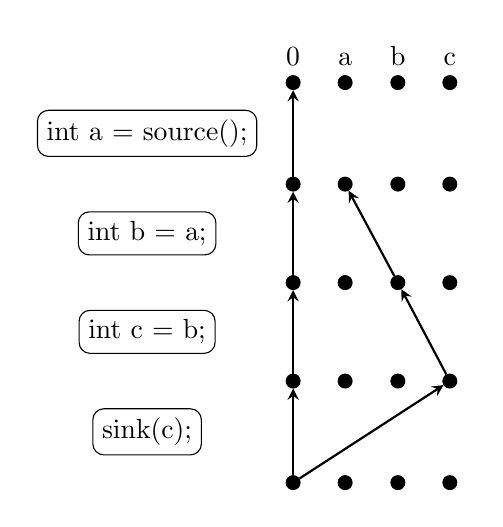
\begin{tikzpicture}[auto,
                s/.style={draw, rounded corners},
                v/.style={draw, fill=black, circle, inner sep=0pt, minimum size=5pt},
                every node/.style={align=center},
                every matrix/.style={ampersand replacement=\&,column sep=0.25cm,row sep=.25cm},
                vto/.style={->, >=stealth, thick}]
                \matrix {
                    \& \node[v, label=0] (zero1) {}; \& \node[v, label=a] (a1) {}; \& \node[v, label=b] (b1) {}; \& \node[v, label=c] (c1) {};\\
                    \node[s] (s1) {\smallcode{int a = source();}}; \& \& \& \&\\
                    \& \node[v] (zero2) {}; \& \node[v] (a2) {}; \& \node[v] (b2) {}; \& \node[v] (c2) {};\\
                    \node[s] (s2) {\smallcode{int b = a;}}; \& \& \& \&\\
                    \& \node[v] (zero3) {}; \& \node[v] (a3) {}; \& \node[v] (b3) {}; \& \node[v] (c3) {};\\
                    \node[s] (s3) {\smallcode{int c = b;}}; \& \& \& \&\\
                    \& \node[v] (zero4) {}; \& \node[v] (a4) {}; \& \node[v] (b4) {}; \& \node[v] (c4) {};\\
                    \node[s] (s4) {\smallcode{sink(c);}}; \& \& \& \&\\
                    \& \node[v] (zero5) {}; \& \node[v] (a5) {}; \& \node[v] (b5) {}; \& \node[v] (c5) {};\\
                };

                \draw[vto] (zero5) -- (zero4);
                \draw[vto] (zero4) -- (zero3);
                \draw[vto] (zero3) -- (zero2);
                \draw[vto] (zero2) -- (zero1);

                \draw[vto] (zero5) -- (c4);
                \draw[vto] (c4) -- (b3);
                \draw[vto] (b3) -- (a2);
            \end{tikzpicture}
            \caption{Backward}
            \label{tikz:rtol_b}
        \end{subfigure}
        \caption{Right-to-Left Order}
        \label{tikz:rtol}
    \end{figure}

    \begin{figure}[tbp]
        \centering
        \begin{subfigure}[b]{\textwidth}
            \begin{lstlisting}[gobble=16]
                StringBuilder sb = new StringBuilder();
                sb = sb.append("DeviceID: ").append(id).append("\n IMEI: ")
                    .append(imei).append("\n ISMI: ").append(imsi);
            \end{lstlisting}
            \caption{Java}
        \end{subfigure}
        \qquad
        \begin{subfigure}[b]{\textwidth}
            \begin{lstlisting}[language=Jimple, gobble=16]
                $stack9 = new java.lang.StringBuilder;
                specialinvoke $stack9.<java.lang.StringBuilder: void <init>()>();
                $stack10 = virtualinvoke $stack9.<java.lang.StringBuilder: java.lang.StringBuilder append(java.lang.String)>("My device id is ");
                $stack11 = virtualinvoke $stack10.<java.lang.StringBuilder: java.lang.StringBuilder append(java.lang.String)>($stack6);
                $stack12 = virtualinvoke $stack11.<java.lang.StringBuilder: java.lang.StringBuilder append(java.lang.String)>(",my IMEI is ");
                $stack13 = virtualinvoke $stack12.<java.lang.StringBuilder: java.lang.StringBuilder append(int)>($stack7);
                $stack14 = virtualinvoke $stack13.<java.lang.StringBuilder: java.lang.StringBuilder append(java.lang.String)>(" and my IMSI is ");
                $stack15 = virtualinvoke $stack14.<java.lang.StringBuilder: java.lang.StringBuilder append(int)>($stack8);
            \end{lstlisting}
            \caption{Jimple}
        \end{subfigure}
        \caption{StringBuilder example}
        \label{lst:stringbuilder}
    \end{figure}

    We already briefly mentioned the global scope of static field taints in the \hyperref[s:rules]{last section}.
    Hence, unless the static taint is overwritten, it traverses the whole interprocedural control-flow graph.
    This obviously creates many unneccessary edges. \textsc{FlowDroid} already applies an optimization and looks ahead to skip methods in which the static field is not used.
    Still, the long lifetime stays an issue for real-world application and the direction can not generally change this issue \cite{Arzt2017PhD}.

    We discussed the complexity based on the taint propagations.
    However, they are only known after the analysis.
    Now, it would be beneficial to decide which direction is the best before analyzing an app.
    An obvious choice for a clue would be the ratio of sources and sinks.
    If one is much less than the other, we could argue less taints to start with should also lower the taint propagations.
    Sadly, it is not as easy to generalize the statement to less starting taints means less runtime.
    Arzt's evaluation of \textsc{FlowDroid} has shown no correlation between the number of sources and the runtime in \textsc{FlowDroid}\cite{Arzt2017PhD}.
    This result indicates that the observed statements have way more influence on the number of taint propagations balancing out the initial advantage.
    Even though the starting taints possibly do not correlate with the runtime, whenever there is a tiny number of sinks but hundreds of sources, the backward analysis should perform better.
    Likewise, Lerch et al. claim in their work that a magnificent smaller amount of sinks than sources are advantageous for a backward-directed search \cite{Lerch2014}.

    The choice on the direction might also be useful for special analysis applications.
    Think of a case where sanitization methods\footnotemark{} are in use.
    \footnotetext{Sanitization methods are run against user input to ensure the input is safe to be processed.}
    Depending on the use case, it might be possible to deduce the proximity between sanitization methods and sources or sinks.
    Whenever this is possible, there should be a clear favorite for one direction due to the taints' lower lifetime.

    % Summarized, we discussed cases where one direction seems favorable, but no generalized statement can be made on which analysis direction is better. Further, most of the influencing factors depend on the app and thus, at most, a favorable direction can be determined for a single app.
\end{document}